%! suppress = EscapeHashOutsideCommand
%! Author = Theodore Capinski
%! Date = 3/13/2024

% Preamble
\documentclass[11pt]{article}
\let\oldsection\section
\renewcommand\section{\clearpage\oldsection}
\setcounter{section}{-1}
\counterwithin{figure}{section}

% Packages
\usepackage{amsmath}
\usepackage{hyperref}
\usepackage{graphicx}
\usepackage{tikz}
\usepackage{indentfirst}
\usepackage{circuitikz}
\usepackage{calc}
\usepackage{float}

%%%%%%%%%%%%%%%%%%%%%%%%%%%%%%%%%%%%%%%%%%%%%%%%%%%%%%%%%%%%%%%%%%%%%%
% LaTeX Overlay Generator - Annotated Figures v0.0.1
% Created with http://ff.cx/latex-overlay-generator/
%%%%%%%%%%%%%%%%%%%%%%%%%%%%%%%%%%%%%%%%%%%%%%%%%%%%%%%%%%%%%%%%%%%%%%
%\annotatedFigureBoxCustom{bottom-left}{top-right}{label}{label-position}{box-color}{label-color}{border-color}{text-color}
\newcommand*\annotatedFigureBoxCustom[8]{\draw[#5,thick,rounded corners] (#1) rectangle (#2);\node at (#4) [fill=#6,thick,shape=circle,draw=#7,inner sep=2pt,font=\sffamily,text=#8] {\textbf{#3}};}
%\annotatedFigureBox{bottom-left}{top-right}{label}{label-position}
\newcommand*\annotatedFigureBox[4]{\annotatedFigureBoxCustom{#1}{#2}{#3}{#4}{white}{white}{black}{black}}
\newcommand*\annotatedFigureText[4]{\node[draw=none, anchor=south west, text=#2, inner sep=0, text width=#3\linewidth,font=\sffamily] at (#1){#4};}
\newenvironment {annotatedFigure}[1]{\centering\begin{tikzpicture}
                                                   \node[anchor=south west,inner sep=0] (image) at (0,0) { #1};\begin{scope}[x={(image.south east)},y={(image.north west)}]}{\end{scope}\end{tikzpicture}}
%%%%%%%%%%%%%%%%%%%%%%%%%%%%%%%%%%%%%%%%%%%%%%%%%%%%%%%%%%%%%%%%%%%%%%

\newcommand{\todo}[1]{\textcolor{red}{TODO: #1}\PackageWarning{TODO:}{#1!}}

\title{Physics 5BL Lab Report RC Circuits}
\author{T.~Capinski \and A.~Patel}

% Document
\begin{document}
    \maketitle
    \tableofcontents

    \section*{Introduction}\label{sec:introduction}
    \addcontentsline{toc}{section}{Introduction}

    In this lab, we will be studying the behavior of simple RC and RLC circuits.
    We will find the time constant of an RC circuit and the resonant frequency of an RLC circuit.
    The circuits will be driven by a function generator, and the voltage across the capacitor or inductor will be measured with an oscilloscope.

    \todo{Check if this is right after part 1 is finished}
    In part 1, we measured the time constant of an RC circuit with a 10 k$\Omega$ resistor and a capacitor with a capacitance of 47 μF. We found that our time constant was $\tau = 1 \times 10^{3} \times 47 \times 10^{-6} = 47$ ms. This was inside the range of accepted values. We also created our own capacitors in this section, trying to make the capacitance as large as possible. For Patels capacitor, we found the capacitance to be $9.49e*10^{-7} \divided 1 \times 10^{6} = 0.949$ F\@.
    \todo{put in Capinski capacitor and agreement test if done}

    In part 2, we measured the transient behavior of an RLC circuit. The first circuit was underdamped and was composed of a 100 mH inductor, 0.1 µF capacitor, and a 50 $\Omega$ resistor. We then fit our data to a general equation and found the experimental values of $\alpha$ and $\omega_0$ to be 870.141 +/- 31.419 and 9745.214 +/- 101.194 respectively. Our value for ω0 is inside our range of accepted values, however, our value for α is outside our accepted range. The second circuit was overdamped and was composed of a 100 mH inductor, 47 µF capacitor, and a 10 k$\Omega$ resistor. We then fit our data to a general equation and found the experimental value of $\alpha$ to be 1518.932 +/- 30.657, which fell outside the range of accepted values.

    \section*{Theory}\label{sec:theory}
    \addcontentsline{toc}{section}{Theory}

    The capacitance of a capacitor is defined by the equation
    \begin{equation}
        C = \frac{Q}{V}
    \end{equation}\label{eq:capacitance}
    where $C$ is the capacitance, $Q$ is the charge stored on the capacitor, and $V$ is the voltage across the capacitor.

    With the parallel plate capacitor, which we use in our circuits the capacitance is given by
    \begin{equation}
        C = \frac{\varepsilon_r \varepsilon_0 A}{d}
    \end{equation}\label{eq:parallel-plate-capacitance}
    where $\varepsilon_r$ is the relative permittivity of the dielectric, $\varepsilon_0$ is the vacuum permittivity, $A$ is the area of the plates, and $d$ is the separation between the plates.

    The charge in a discharging capacitor is given by
    \begin{equation}
        Q(t) = Q_0 e^{-t/RC}
    \end{equation}\label{eq:discharging-capacitor}
    with RC being the time constant of the circuit, $\tau$.

    An RLC circuit requires different paramters to be defined.
    The resonant frequency of an RLC circuit is calculated with
    \begin{equation}
        \omega_0 = \frac{1}{\sqrt{LC}}
    \end{equation}\label{eq:omega-0}
    where $L$ is the inductance, and $C$ is the capacitance.
    A factor of inverse time constant is given by
    \begin{equation}
        \alpha = \frac{R}{2L}
    \end{equation}\label{eq:alpha}

    This allows the circuit to be analyzed as damped, underdamped, or overdamped, using the ratio $\frac{\alpha}{\omega_0}$.
    The frequency is thus given by
    \begin{equation}
        \omega = 2\pi f
    \end{equation}\label{eq:frequency}

    We can also define another equation for ${\omega}$ using ${\omega_0}$ and ${\alpha}$:
    \begin{equation}
        \omega = \sqrt{\omega_0^2 - \alpha^2}
    \end{equation}\label{eq:omega}

    In part 2A, we will fit our data to the following equation for current:

    \begin{equation}
        I = Ae^{-\alpha t} \cos(\omega t - \phi)
    \end{equation}\label{eq:current_2a}
    Where I is current, A is the overall oscillation amplitude and $\phi$ is the phase angle.

    The voltage across a discharging capacitor in an RLC circuit (part 2B) should fit the equation
    \begin{equation}
        V(t)/v0 = A e^{-t/B}
    \end{equation}\label{eq:capacitor-voltage}
    where $A$ is the initial voltage, and $B$ is the time constant.

    We will also need an agreement test to compare our experimental values to the theoretical values.
    The agreement test is given by
    \begin{equation}
        |x_{\text{exp}} - x_{\text{theo}}| \le 2 \sqrt{\sigma_{\text{exp}}^2 + \sigma_{\text{theo}}^2}
    \end{equation}\label{eq:agreement-test}

    \section{Part 1: Time Constant With Oscilloscope}\label{sec:measuring-time-constant}

    \subsection{Methods}\label{subsec:measuring-time-constant-methods}

    The first experiment was to measure the time constant of an RC circuit.
    The circuit was set up as shown in Figure\ref{fig:rc-circuit}.
    The function generator was set to produce a square wave with a frequency of 100 mHz and a peak-to-peak voltage of 10 V.
    The voltage across the capacitor was measured with an oscilloscope.

    \begin{figure}[H]
        \begin{center}
            \begin{circuitikz}[american]
                \draw (0,0) to [sV=$V_1$] ++ (0,2)
                to [R=$R$] ++ (2,0)
                to [C=$C$] ++ (2, 0)
                -- ++ (0,-2)
                -- ++ (-4,0);
            \end{circuitikz}
        \end{center}
        \caption{RC Circuit}
        \label{fig:rc-circuit}
    \end{figure}

    First, the time constant was found with a known resistor and capacitor.
    Afterward, we constructed a capacitor using aluminum foil and paper, and measured the time constant with a larger resistor.
    Again, the resistance was known, and the capacitance was estimated from the area and separation of the plates.

    Our data collection procedure was simple.
    We paused the oscilloscope with a full period of the square wave input visible.
    We then used the cursor to record around 10-15 data points of the voltage across the capacitor.
    We recorded the time and voltage of each point.

    \begin{figure}[H]
        \begin{annotatedFigure}
            {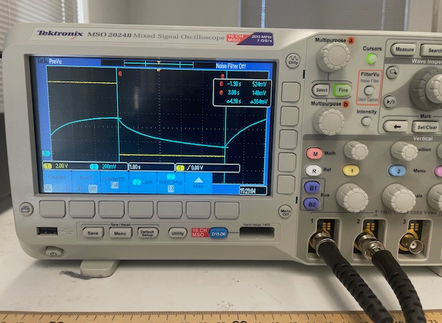
\includegraphics[width=1.0\linewidth]{resources/images/rlc part 1 oscilliscope}}
            \annotatedFigureBox{0.015,0.15}{0.963,0.9338}{A}{0.015,0.15}%bl
            \annotatedFigureBox{0.053,0.3828}{0.647,0.8489}{B}{0.053,0.3828}%bl
        \end{annotatedFigure}
        \caption{The oscilloscope display of the RC circuit. (A) is the machine, and (B) is the display showing the graph of the voltage across the capacitor.}
        \label{fig:part1_oscilloscope}
    \end{figure}

    \subsection{Analysis}\label{subsec:measuring-time-constant-analysis}

    The data was then analyzed by fitting the voltage across the capacitor to the equation for a discharging capacitor.
    The time constant was then calculated from the fit.

    To fit the data, we used Equation~\ref{eq:discharging-capacitor}.
    We found the best fit parameters for the amplitude $A$ and the time constant $B$.

    For the known capacitor, Figure~\ref{fig:part1a_graph} shows the voltage across the capacitor discharging over time.

    \begin{figure}[H]
        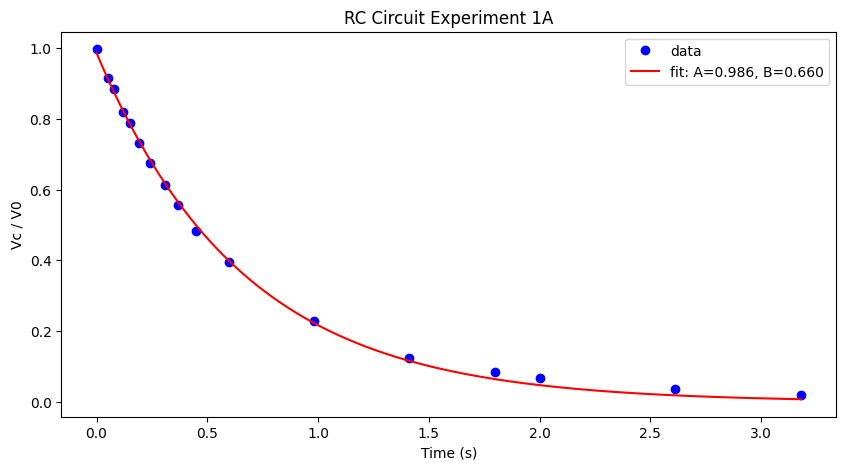
\includegraphics[width=1.0\linewidth]{resources/images/rc part 1a graph}
        \caption{The voltage across the capacitor in the RC circuit.}
        \label{fig:part1a_graph}
    \end{figure}

    The theoretical time constant was calculated using the known values of the resistor and capacitor.
    Using equation~\ref{eq:capacitance}, we found the theoretical time constant to be $\tau = 1 \times 10^{3} \times 47 \times 10^{-6} = 47$ ms.
    The data resulted in the fit values $A = 0.986 \pm 0.006$ V and $B = 0.660 \pm 0.011$ s.
    Using the agreement test from Equation~\ref{eq:agreement-test}, we found that the theoretical value was within the range of the experimental value.

    \begin{e}
        \begin{align*}
        |47 - 660| \le2 \sqrt{6^2 + 11^2} \\
        613 \le25.06
        \end{align*}
    \end{e}
    \todo{Check the agreement test calculation.}

    Since the time constant agreed with the theoretical value, we concluded that the circuit was functioning as expected.
    This meant that we could trust the measured time constant value for when we constructed our own capacitor.

    For the handcrafted capacitor, we found the time constant with the same procedure.
    We measured each of our capacitors.
    The fit is shown in Figure~\ref{fig:part1b_graph_patel}.
    \todo{show residuals}
    \todo{add capinski data}

    \begin{figure}[H]
        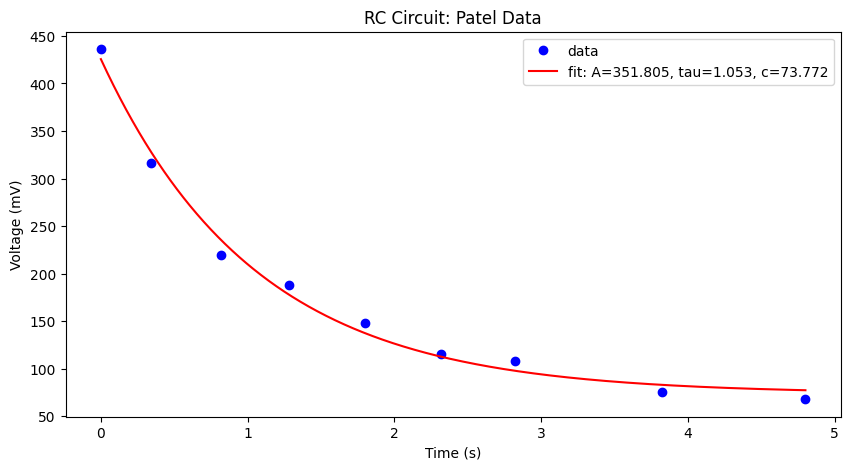
\includegraphics[width=1.0\linewidth]{resources/images/rc part 1 graph patel}
        \caption{The voltage across the capacitor in the RC circuit with the handcrafted capacitor by Patel.}
        \label{fig:part1b_graph_patel}
    \end{figure}

    For Patel's capacitor, the time constant was found to be $9.49e*10^{-7} \pm ???$ s.
    The resistance is known to be 1 M$\Omega$.
    Using equation\ref{eq:capacitance}, we found the capacitance to be $9.49e*10^{-7} \divided 1 \times 10^{6} = 0.949$ F\@.
    \todo{agreement test with expected value}

    \subsection{Conclusion}\label{subsec:part1_conclusion}


    \section{Part 2A: RLC Underdamped Transient Response}\label{sec:part2a_underdamped}
    \subsection{Methods}\label{subsec:part2a_methods}
    This section covers the first part of experiment 2, which uses an RLC Circuit to find the underdamped transient response. We used a 100 mH inductor, 0.1 µF capacitor, and a 50 Ω resistor (two 100 Ω resistors in parallel), as seen in the following diagram:
    
    \begin{figure}[h]
    \centering
    \begin{circuitikz}
        \draw (0,0) to[battery1, l=$V$] (0,2)
                    to[inductor, l=$L$] (2,2)
                    to[capacitor, l=$C$] (4,2)
                    -- (6,2)
                    to[R, l=$R$] (6,0)
                    -- (4,0)
        \draw (6,2) to[R, l=$R$] (8,2)
                    -- (8,0)
                    -- (6,0)
                    -- (0,0);
    \end{circuitikz}
    \caption{Circuit setup for parts 2a and 2b}
    \end{figure}

    We also used the function generator to create a signal. We used a 10 Hz square wave with 4 Vpp and an output impedance of 50 Ω. We saw the following wave on our oscilloscope:

    todo - picture of part 2a graph
    caption: Graph from experiment 2a

    We then recorded the peaks of the wave and recorded them in the following data table:

    \begin{table}[h]
        \centering
        \caption{Time and Voltage Measurements Part 2A}
        \begin{tabular}{cc}
            \toprule
            \textbf{Time (ms)} & \textbf{Volts (mV)} \\
            \midrule
            0.00 & 3.97 \\
            0.16 & -176 \\
            0.48 & 136 \\
            0.81 & -96 \\
            1.14 & 72 \\
            1.464 & -56 \\
            1.764 & 48 \\
            2.144 & -32 \\
            2.464 & 24 \\
            2.808 & -16 \\
            3.088 & 8 \\
            \bottomrule
        \end{tabular}
    \end{table}



    \subsection{Analysis}\label{subsec:part2a_analysis}
    We divided each voltage we obtained by the effective resistance (125 $\Omega$) in order to fit it to the current equation, although its important to note that this only changes the amplitude. We graphed the new data points and fit them to equation~\ref{eq:current_2a}. We obtained the following graph and its residuals:

    todo input part 2a graph and residuals
    caption for graph: Underdamped RLC Circuit data and fit
    caption for residuals: Underdamped RLC Circuit residuals

    From this, we can see that our value for x (\( \alpha \)) is 870.141 +/- 31.419 and w (\( \omega \)) is 9706.289 +/- 101.561. Solving for \( \omega_0 \) using equation ~\ref{eq:omega}, we get 9745.214 +/- 101.194. When we solve for those values using theoretical values and the equations~\ref{eq:alpha} and ~\ref{eq:omega-0}, we get the values:

    \begin{align*}
        \alpha &= \frac{125}{2 \times 0.1} = 625
    \end{align*}

    \begin{align*}
        \omega &= \frac{1}{\sqrt{0.1^2 \times 10^{-6}}} = \frac{1}{0.1 \times 10^{-3}} = 10000
    \end{align*}

    We can clearly see a difference in our values for \( \alpha \) and \( \omega_0 \), but they are reasonable. We can do an agreement test from equation~\ref{eq:agreement-test} to test our values for \( \omega_0 \) and \( \alpha \) respectively.

    \begin{e}
        \begin{align*}
            |9745.214 - 10000| &\le 2 \sqrt{100^2 + 101.194^2} \\
            245.786 &\le 2 \sqrt{20240.226} \\
            245.786 &\le 284.536
        \end{align*}
    \end{e}
    \begin{e}
        \begin{align*}
            |870.141 - 625| &\ge 2 \sqrt{62.5^2 + 31.419^2} \\
            245.141 &\ge 2 \sqrt{4893.404} \\
            245.141 &\ge 139.904
        \end{align*}
    \end{e}

    As we can see, our value for \( \omega_0 \) is inside our range of accepted values and thus we consider it reasonable. However, our value for \( \alpha \) is outside our accepted range. This could be due to our measured circuit resistance being lower than it actually was. Our measurement error could also have been too low, resulting in a low error and a value outside an accepted range. External factors such as temperature variations or electromagnetic interference from other groups' experiments could also have influenced the circuit's behavior.


    \section{Part 2B: RLC Overdamped Transient Response}\label{sec:part2b_overdamped}
    \subsection{Methods}\label{subsec:part2b_methods}
    This section covers the second part of experiment 2, which uses an RLC Circuit to find the overdamped transient response. We used a 100 mH inductor, 47 µF capacitor, and a 10 kΩ resistor, as seen in the following diagram:

    todo - picture of part 2b circuit
    caption: Circuit setup for part 2b

    We also used the function generator to create a signal. We used a 50 Hz square wave with 4 Vpp and an output impedance of 50 Ω. We saw the following wave on our oscilloscope:

    todo - picture of part 2b graph
    caption: Graph from experiment 2b

    We then recorded the peaks of the wave and recorded them in the following data table:

    \begin{table}[h]
        \centering
        \caption{Time and Voltage Measurements Part 2B}
        \begin{tabular}{cc}
            \toprule
            \textbf{Time (ms)} & \textbf{Volts (V)} \\
            \midrule
            0.00 & 3.96 \\
            0.16 & 3.08 \\
            0.28 & 2.52 \\
            0.44 & 1.96 \\
            0.64 & 1.48 \\
            0.80 & 1.16 \\
            0.96 & 0.92 \\
            1.16 & 0.68 \\
            1.60 & 0.44 \\
            2.04 & 0.20 \\
            3.76 & 0.12 \\
            5.20 & 0.04 \\
            \bottomrule
        \end{tabular}
    \end{table}


    \subsection{Analysis}\label{subsec:part2b_analysis}
    We divided each voltage we obtained by the input volgtage (4 V) in
    order to fit it to our equation, although its important to note that
    this only changes the amplitude. We graphed the new data points and fit
    them to equation ~\ref{eq:capacitor-voltage}. We obtained the following
    graph and its residuals:

    todo input part 2b graph and residuals
    caption for graph: overdamped RLC Circuit data and fit
    caption for residuals: overdamped RLC Circuit residuals

    From this, we can see that our graph is a good fit, as it goes through or close to all the points. The residuals are also randomly scattered around the 0 line. Our value for A is 0.980 +/- 0.011 and D is 1518.932 +/- 30.657. When we solve for \( \alpha \), it is unnecessary to account for the resistance from the inductor, since the resistor is much larger than the resistance the inductor will provide, allowing us to consider it negligible. Calculating \( \alpha \) using theoretical values and the equation~\ref{eq:alpha}, we get the value:

    \[
        \alpha = \frac{10000}{2 \times 0.1} \\ = 50{,}000
    \]

    We can clearly see a large difference in our value for \( \alpha \). We can do an agreement test from equation ~\ref{eq:agreement-test} to test our value for \( \alpha \).

    \begin{e}
        \begin{align*}
            |1518.932 - 50000| &\ge 2 \sqrt{30.657^2 + 500^2} \\
            48481.068 &\ge 2 \sqrt{250939.852} \\
            48481.068 &\ge 500.93897
        \end{align*}
    \end{e}

    As we can see, our value for \( \alpha \) is very far outside our accepted range. This could be due to our measured circuit resistance being lower than it actually was. The damping ratio in an RLC circuit could also vary depending on the frequency of the input signal. At certain frequencies, the circuit might exhibit more pronounced oscillations due to resonance effects, resulting in a lower damping ratio. Also, any additional sources of energy loss in the circuit, such as resistance in the connections, stray capacitance, or inductance, could have contributed to the lower value for \( \alpha \).


    \section{Part 2 Conclusion}\label{sec:part2_conclusion}
    In part 2 of this lab, we designed 2 experiments using an RLC circuit. They both used different values for the capacitor and resistor, however, we kept the inductor at 100 mH.

    In part A, we used a  0.1 µF capacitor and a 50 $\Omega$ resistor in order to get an underdamped transient response. We then fit our data to equation~\ref{eq:current_2a}, making sure to account for the fact that this is an equation for currently by dividing our voltages by the total resistance. We found the fit parameters $\alpha$ = 870.141 +/- 31.419 and $\omega_0$ = 9706.289 +/- 101.561. We found that our frequency was in the range of the accepted values, calculated from the theoretical values, however, our value for $\alpha$ was outside the range. This could have been due to our measured circuit resistance being lower than it actually was or electromagnetic interference from other groups’ experiments.

    In part B, we used a 47 µF capacitor and a 10k $\Omega$ resistor in order to get an overdamped transient response. We then fit our data to equation~\ref{eq:capacitor-voltage}. We found the fit parameters A = 0.980 +/- 0.011 and D = 1518.932 +/- 30.657. We focused on our value for D, comparing it to the theoretical value for $\alpha$, calculated using equation~\ref{eq:alpha}. We found that our value was outside the acceptable range of values. This error could have been due to our measured circuit resistance being lower than it was, or the damping ratio in an RLC circuit varying depending on the frequency of the input signal.

    \section{Lab Conclusion}\label{sec:conclusion}
    In this lab, we learned about RC circuits and how to study the time-dependent behavior of both RC and RLC circuits with a DC source and build a capacitor. We also learned about RLC circuits and how to measure the transient response of an underdamped and overdamped circuit. We explored charging and discharging behaviors of RC series circuits and constructed our own capacitors with household materials and measured its capacitance. We then explored the transient behavior of RLC circuits and their under and overdamped properties.

    Part 1A involved setting up an RC circuit with a square wave input from a function generator, measuring the discharge curve across the capacitor using an oscilloscope in roll mode, and determining the time constant by analyzing the decay curve. We adjusted the oscilloscope settings to capture the decay over at least 5 time constants and utilized cursors to measure voltage drops and decay times accurately, ensuring a comprehensive understanding of the circuit's behavior.

    In Part B, we constructed homemade capacitors by sandwiching aluminum foil between pieces of paper, aiming to maximize capacitance. We then connected these capacitors in an RC circuit with a 1 MΩ resistor to measure their capacitance using charging and discharging curves on the oscilloscope. Despite theoretical estimations, our practical capacitance values differed, likely due to imperfections in construction and contact losses.

    Experiment 2A involved exploring the underdamped transient response of an RLC circuit. We observed the damped ringing behavior in the voltage across the resistor using an oscilloscope, recording peak amplitudes and their time relative to the square wave input pulse for analysis. By performing a fit to the underdamped current behavior equation, we determined experimental values for the damping coefficient and the natural frequency comparing them with theoretical values to assess agreement.

    In Experiment 2B, we investigated the overdamped transient response of an RLC circuit. We observed the decay of the waveform and characterized the decay constant by obtaining sufficient data points. Using a direct non-linear fit, we determined the experimental decay time constant and compared it with theoretical values to evaluate agreement.

    Overall, the experiments went into the transient behaviors of RLC circuits, exploring underdamped and overdamped regimes. Through practical setups, data acquisition, and analysis, we gained a deeper understanding of the characteristics and properties of RC and RLC circuits, and got valuable practice using the oscilloscope and experimental equipment.



    \appendix
    \section{References}\label{sec:references}

    Lab Manual


\end{document}